\pdfminorversion=4
\documentclass[aspectratio=169]{beamer}

\mode<presentation>
{
  \usetheme{default}
  \usecolortheme{default}
  \usefonttheme{default}
  \setbeamertemplate{navigation symbols}{}
  \setbeamertemplate{caption}[numbered]
  \setbeamertemplate{footline}[frame number]  % or "page number"
  \setbeamercolor{frametitle}{fg=white}
  \setbeamercolor{footline}{fg=black}
} 

\usepackage[english]{babel}
\usepackage[utf8x]{inputenc}
\usepackage{tikz}
\usepackage{courier}
\usepackage{array}
\usepackage{bold-extra}
\usepackage{minted}
\usepackage[thicklines]{cancel}
\usepackage{fancyvrb}

\xdefinecolor{dianablue}{rgb}{0.18,0.24,0.31}
\xdefinecolor{darkblue}{rgb}{0.1,0.1,0.7}
\xdefinecolor{darkgreen}{rgb}{0,0.5,0}
\xdefinecolor{darkgrey}{rgb}{0.35,0.35,0.35}
\xdefinecolor{darkorange}{rgb}{0.8,0.5,0}
\xdefinecolor{darkred}{rgb}{0.7,0,0}
\definecolor{darkgreen}{rgb}{0,0.6,0}
\definecolor{mauve}{rgb}{0.58,0,0.82}

\title[2019-04-19-coffea-review]{Perspective on Coffea from IRIS-HEP}
\author{Jim Pivarski}
\institute{Princeton University -- IRIS-HEP}
\date{April 19, 2019}

\usetikzlibrary{shapes.callouts}

\begin{document}

\logo{\pgfputat{\pgfxy(0.11, 7.4)}{\pgfbox[right,base]{\tikz{\filldraw[fill=dianablue, draw=none] (0 cm, 0 cm) rectangle (50 cm, 1 cm);}\mbox{\hspace{-8 cm}
\includegraphics[height=1 cm]{princeton-logo-long.png}\hspace{0.1 cm}\raisebox{0.1 cm}{
\includegraphics[height=0.8 cm]{iris-hep-logo-long.png}}\hspace{0.1 cm}}}}}

\begin{frame}
  \titlepage
\end{frame}

\logo{\pgfputat{\pgfxy(0.11, 7.4)}{\pgfbox[right,base]{\tikz{\filldraw[fill=dianablue, draw=none] (0 cm, 0 cm) rectangle (50 cm, 1 cm);}\mbox{\hspace{-8 cm}
\includegraphics[height=1 cm]{princeton-logo.png}\hspace{0.1 cm}\raisebox{0.1 cm}{
\includegraphics[height=0.8 cm]{iris-hep-logo.png}}\hspace{0.1 cm}}}}}

% Uncomment these lines for an automatically generated outline.
%\begin{frame}{Outline}
%  \tableofcontents
%\end{frame}

% START START START START START START START START START START START START START

\begin{frame}{IRIS-HEP}
\vspace{0.17 cm}
\begin{columns}
\column{1.2\linewidth}
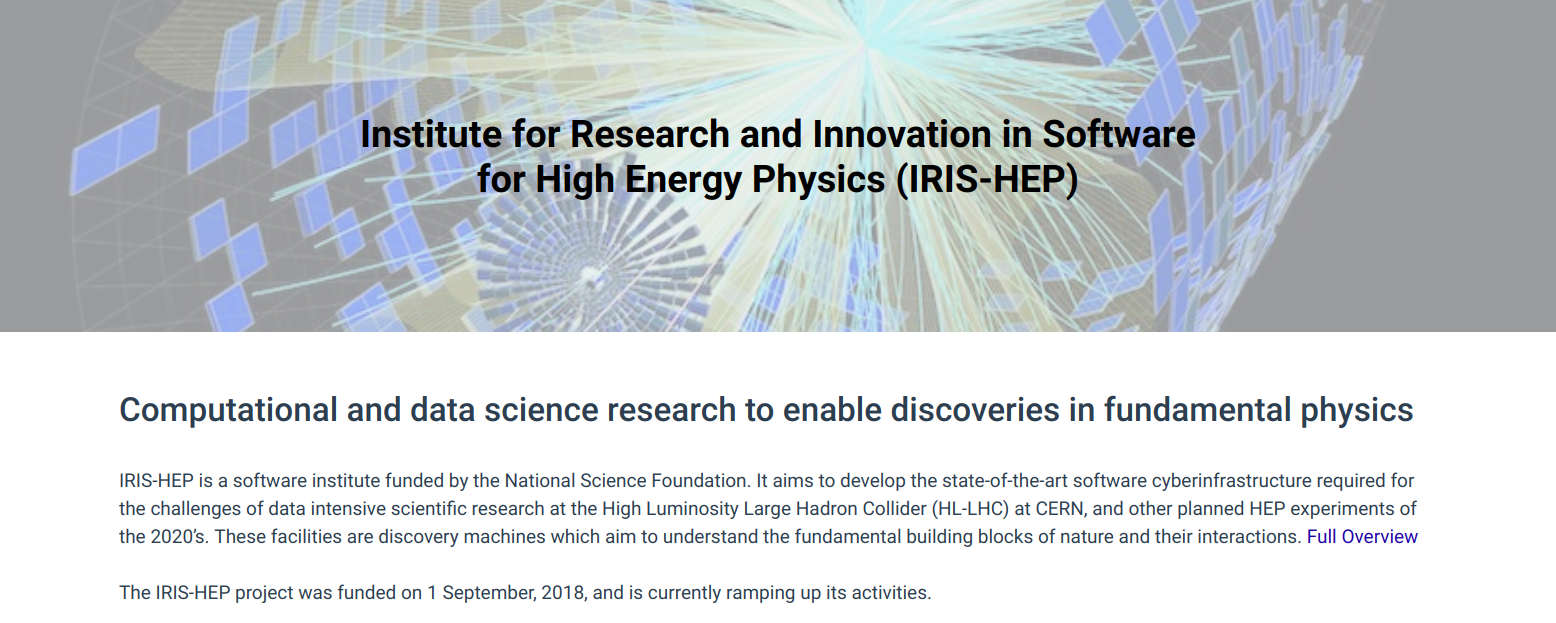
\includegraphics[width=\linewidth]{iris-hep-top.png}


\includegraphics[width=\linewidth]{iris-hep-bot.png}
\end{columns}
\end{frame}

\begin{frame}{IRIS-HEP Analysis Systems}
\begin{columns}[t]
\column{0.5\linewidth}

{\large NYU: Kyle Cranmer}

Statistics, analysis reinterpretation, full-workflow portability

\vspace{0.2 cm}
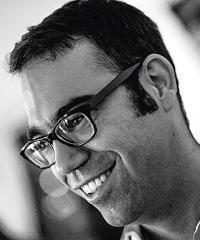
\includegraphics[height=1.5 cm]{Kyle-Cranmer.jpg}

\vspace{0.5 cm}
{\large UW: Gordon Watts, Emma Torro, Mason Proffitt}

Analysis language/\only<1>{expressing queries}\only<2>{\textcolor{darkblue}{expressing queries}}

\vspace{0.2 cm}
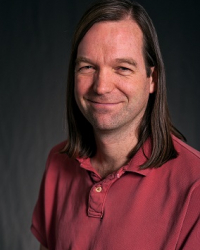
\includegraphics[height=1.5 cm]{Gordon-Watts.jpg}
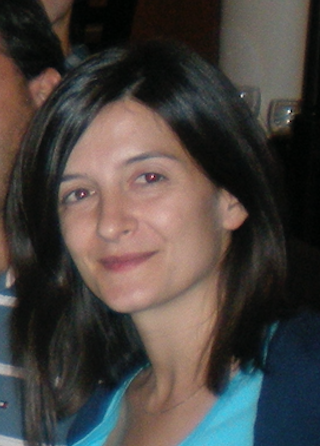
\includegraphics[height=1.5 cm]{ETorro.png}
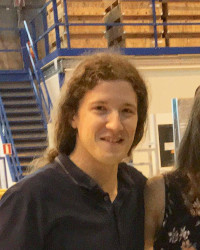
\includegraphics[height=1.5 cm]{Mason-Proffitt.jpg}

\column{0.5\linewidth}

{\large Illinois: Mark Neubauer, Ben Galewsky}

Data delivery (iDDS) and \only<1>{distributed query execution}\only<2>{\textcolor{darkblue}{distributed query execution}}

\vspace{0.2 cm}
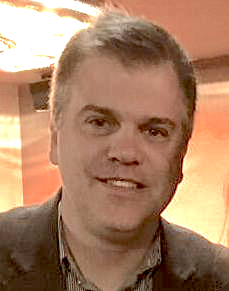
\includegraphics[height=1.5 cm]{Mark-Neubauer.png}

\includegraphics[height=1.5 cm]{Ben-Galewsky.jpg}

\vspace{0.5 cm}
{\large Princeton: Jim Pivarski, Henry Schreiner}

\only<1>{Columnar query execution}\only<2>{\textcolor{darkblue}{Columnar query execution}}, distributed histogramming

\vspace{0.2 cm}

\includegraphics[height=1.5 cm]{Jim-Pivarski.jpg}
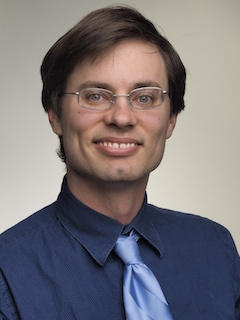
\includegraphics[height=1.5 cm]{Henry-Schreiner.jpg}

\end{columns}
\end{frame}

\begin{frame}{Coffea is tightly connected with analysis software R\&D}
\vspace{0.5 cm}
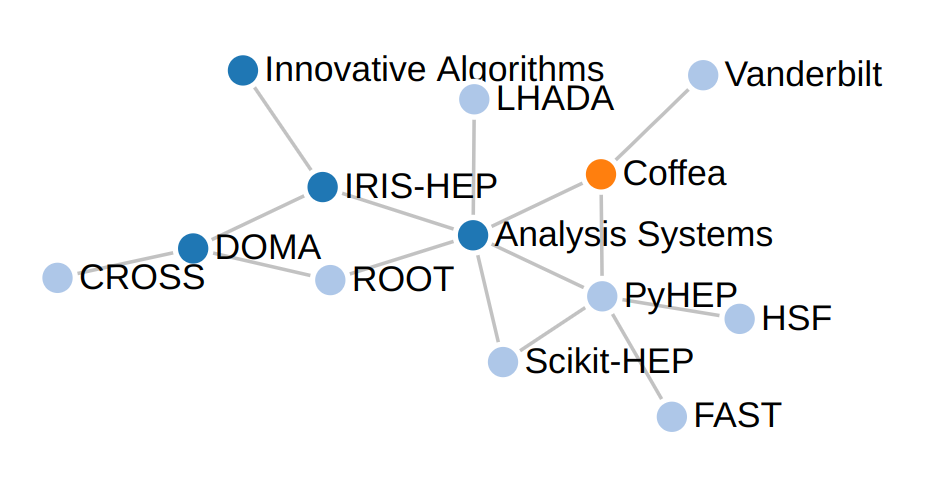
\includegraphics[width=\linewidth]{analysis-connections.png}
\end{frame}

\begin{frame}{Coffea is tightly connected with analysis software R\&D}
\large
\vspace{0.5 cm}
\begin{itemize}\setlength{\itemsep}{0.5 cm}
\item PyHEP/Scikit-HEP (mostly the same people): Coffea uses Pythonic HEP tools and contributes back to the community.
\item IRIS-HEP Analysis Systems: working with Ben Galewsky on Spark scale-out software.
\item IRIS-HEP Analysis Systems: working with me---great feedback!
\item Vanderbilt: working with Andrew Melo on Spark scale-out infrastructure (and software).
\end{itemize}
\end{frame}

\begin{frame}{The value of a real physics use-case can't be overstated}
\Large
\vspace{0.25 cm}
I've been trying to get ``embedded'' with a physics group like this for several years. (For example, XENON-nT.)

\vspace{0.25 cm}



\end{frame}

\end{document}
